Die Entwicklung der nativen Mobilanwendung wird im Folgenden exemplarisch anhand einer \textit{iOS}-Applikation dargestellt. Diese werden ausschließlich auf Mobilgeräten vom U.S.-amerikanischen Hersteller \textit{Apple, Inc.} ausgeführt, funktionieren also auf diversen \textit{iPhone}-, \textit{iPod touch}- und in gewisser Hinsicht auch auf \textit{iPad}-Geräten. Letztere sind wegen der im September 2019 in Kraft getretenen Einführung des sog. \textit{iPadOS} nicht mehr auf reine iOS-Anwendungen ausgelegt, sondern nutzen diese lediglich in Form einer Vergrößerung der Kleingeräteanwendung.

Dieses Kapitel stellt im Folgenden den gesamten Entwicklungsprozess der To-Do-Anwen-dung dar. Der in Abs. \ref{subsec:apple_ios} angesprochene Standard heutiger iOS-Entwicklung wird auch in der Praxis dieser Untersuchung angewandt. Somit fällt die Wahl der Programmiersprache auf Apple Swift 5 unter der \acs{ide} Xcode 11. Im Hinblick auf die To-Do-Anwendung, welche einen persistenten Speicher benötigt, kann hier bereits die Integration der internen Bibliothek \textit{Core Data} hinzugefügt werden.

Grundsätzlich ist es sinnvoll, mit der Gestaltung der visuellen Ansicht zu beginnen, da die erstellten Komponenten im Nachhinein explizit im Quellcode referenziert werden können, um ihnen Funktionalität zu verleihen.

\subsection{Gestaltung des \acl{ui}} \label{subsec:ios_ui}
\subsubsection{Einbinden von \acs{ui}-Komponenten}
Initial beinhaltet das \texttt{Main.storyboard} eine Ansicht, welche bereits mit dem automatisch generierten \texttt{ViewController} verknüpft ist. Diese muss nun mit den in Kapitel \ref{chap:architektur} beschriebenen Komponenten gefüllt werden. Die Listenansicht wird über einen \texttt{UITableView} realisiert. Dieser füllt einen großen Teil der Ansicht aus. Der untere Rand der Ansicht wird mit einem \texttt{UITextField} sowie mit einem \texttt{UIButton} versehen, welcher als \texttt{+}-Symbol konfiguriert wird. Somit ist die hierarchisch höchste Stufe der Ansicht fertiggestellt.

Bislang existiert noch keine Konfiguration der unteren Hierarchiestufe, welche aus den einzelnen Zellen des \texttt{UITableView} besteht. Da diese dem gleichen Aufbau folgen sollen, ist die Definition \textit{einer} \texttt{UITableViewCell} genügend, sodass diese dann für die gesamte Liste verwendet und repliziert werden kann. Diese Zelle beinhaltet erneut ein \texttt{UITextField}, sowie drei \texttt{UIButton}s, welche jeweils mit einem Kreuz-, Häkchen-, und Stern-Symbol konfiguriert werden.

Die Farbgebung der einzelnen Buttons wird nach Maßgabe der Farb-Definition aus Sektion \ref{sec:4-3_ui} als \textit{Tint} der Buttons festgelegt.

Das finale \ac{ui} der To-Do-Anwendung, wie es im Interface Builder dargestellt wird, kann dem folgenden Screenshot entnommen werden.

\begin{figure}[h!]
	\centering
	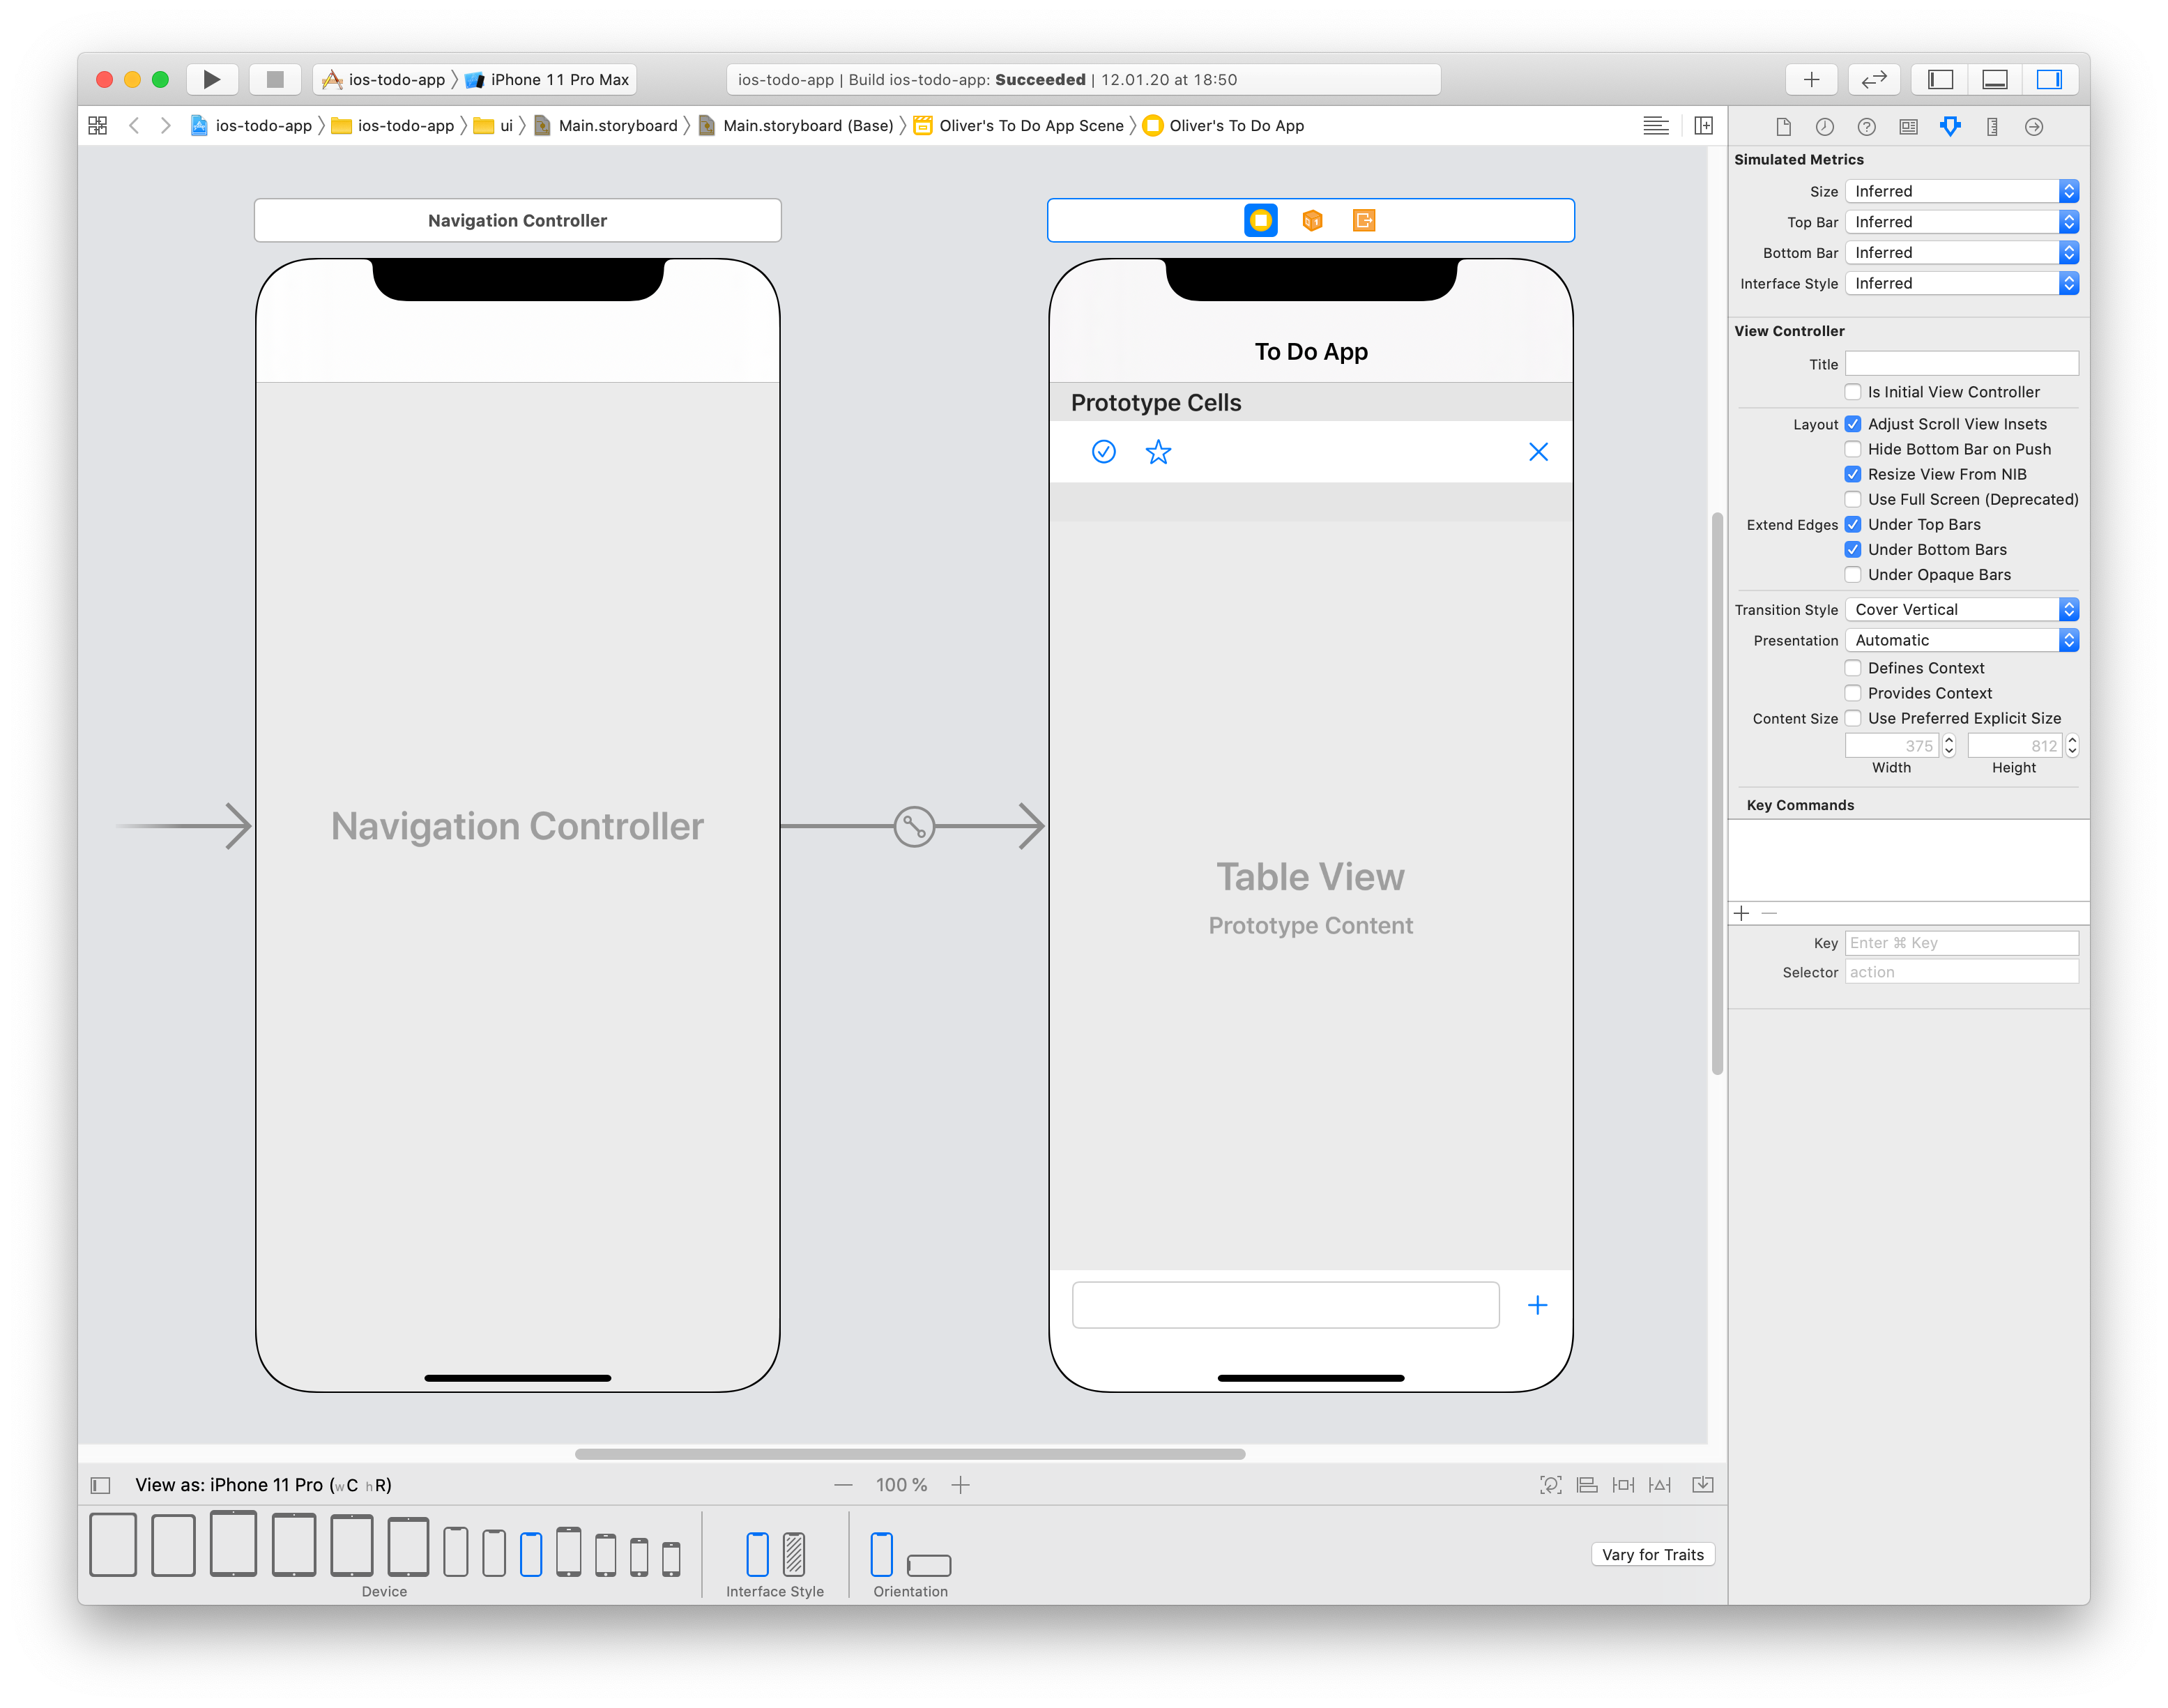
\includegraphics[width=\linewidth]{img/fig/5-1-1_IB_App}
	\caption{\acs{ui} im Interface Builder von Xcode}
	\label{fig:ib-app}
\end{figure}

Der auf der linken Seite sichtbare \textit{Navigation Controller} kann an dieser Stelle vernachlässigt werden, da es nur das Hinzufügen der Kopfleiste mit der Aufschrift \textit{To Do App} zur Folge hat.

\subsubsection{Relative Positionierung der Komponenten}
Apple bietet verschiedene Mobilgeräte in verschiedenen Größen an. Der Interface Builder von Xcode erlaubt die interaktive Positionierung der \ac{ui}-Komponenten jedoch nur unter Betrachtung einer spezifischen Gerätegröße. Wird diese in der Ansicht gewechselt (s. Abb. \ref{fig:ib-app} unten), fällt auf, dass die Positionierung der Komponenten absolut gesetzt wird und diese somit bei kleineren Geräten über den gedachten Bildschirmrand herausgehen bzw. bei größeren Geräten nicht die gesamte Bildschirmbreite ausnutzen.

In vielen Fällen schaffen sog. \textit{Auto-resizing Constraints} Abhilfe gegen dieses Problem. In diesen kann das Verhalten einzelner Komponenten bei bestimmten Bildschirmgrößen bestimmt werden. Dieses Verhalten beschreibt die Änderung der Position sowie der Skalierung der Komponente. So soll der \texttt{UITableView} den gesamten horizontalen Bereich des Bildschirms einnehmen. Gleiches gilt für den Bereich des Textfeldes und des \texttt{+}-Buttons. Da diese jedoch in Abhängigkeit voneinander stehen (d.h. das Textfeld soll immer einen bestimmten Abstand zum Button wahren; der Button soll immer einen bestimmten Abstand zum rechten Bildschirmrand wahren), müssen diese durch eine Unteransicht logisch verbunden werden. In dieser werden dann pixel- oder prozentgenaue Abstände und Änderungen definiert. Diese Unteransicht kann dann wieder über \textit{Auto-resizing Constraints} die gesamte Breite unter der Listenansicht einnehmen. So kann die App nahtlos auf verschieden großen Geräten genutzt werden, ohne dass die Positionierung aller Komponenten für alle möglichen Bildschirmgrößen manuell gesetzt werden muss.

\subsubsection{Dynamische Änderung der Komponentenposition}
Die zuvor definierte Unteransicht, welche für das Erstellen neuer To-Do-Einträge verantwortlich ist, befindet sich zunächst noch jederzeit am unteren Bildschirmrand. Tippt der Nutzer nun in das Textfeld, um einen neuen Eintrag zu erstellen, so werden Textfeld und \texttt{+}-Button von der von unten einfliegenden Tastatur überdeckt. Somit kann der Nutzer seinen Eintrag ins Textfeld nicht sehen und diesen auch nicht über Tippen auf den Button erstellen. Diese Unteransicht muss also bei Aufruf der Tastatur zusammen \textit{mit der Tastatur} verschoben werden.

Auf technischer Ebene muss eine Verschiebung der Unteransicht initiiert werden, sobald die Tastatur zu erscheinen beginnt. Gleichermaßen muss diese Verschiebung rückgängig gemacht werden, sobald die Tastatur wieder verschwindet. Es handelt sich hierbei um \textit{Event Listening} bei einem allgemeinen \ac{ui}-Komponenten, nämlich der Tastatur. Solches Event Listening ist in Swift (noch) nicht abgesehen, weswegen auf Objective-C zurückgegriffen werden muss. Die Listener, auch \textit{Observer}, die auf das Verhalten der Tastatur achten, müssen bei Start der App initialisiert und bei Schließen der App deinitialisiert werden. Sobald einer der Observer über die Änderung des Zustands der Tastatur benachrichtigt, wird die Positionsänderung aufgerufen.

Die absolute Position einer Komponente innerhalb der Ansicht kann anhand eines Koordinatensystems visualisiert werden, welches seinen Ursprung $(0; 0)$ in der oberen linken Ecke hat. Nach rechts hin wächst die $x$-Koordinate, nach unten hin wächst die $y$-Koordinate. Somit muss bei Einfliegen der Tastatur die $y$-Position der Unteransicht um gerade die Höhe der zugrunde liegenden Tastatur reduziert werden, sodass die Unteransicht sich direkt über der Tastatur befindet. Dazu wird zunächst die je nach Sprache variable Tastaturhöhe ermittelt und die $y$-Position um genau diesen Wert reduziert. Um diese Aktion rückgängig zu machen, wird eine Erhöhung der Position um diesen Wert eingeleitet, sobald der entsprechende Observer die Funktion über das Verschwinden der Tastatur benachrichtigt. Die Unteransicht wird nun nicht mehr von der Tastatur verdeckt, sondern wirkt optisch wie ein Teil von ihr, sodass diese nun genutzt werden kann, um To-Do-Einträge zu erstellen. \\\

An dieser Stelle scheint es intuitiv, die Ansicht nun zu testen. Da bislang jedoch noch keinerlei Funktionalität implementiert ist, ist es nun wichtig, Zellen erstellen zu können. Für Testzwecke könnte eine provisorische Funktionsweise entwickelt werden, welche die Zelleninformationen zunächst im Arbeitsspeicher der Anwendung speichert. Da dies jedoch im Nachhinein zu großen Abänderungen des Quellcode-Aufbaus führen kann, werden zunächst der Persistent Service und die \ac{crud}-Funktionen definiert, welche dann direkt über den \texttt{ViewController} an das \ac{ui} angebunden werden.

\subsection{Entwicklung des Persistent Service} \label{subsec:ios_persistent_service}
Wie in Abs. \ref{subsec:apple_ios} erwähnt, geschieht die Konfiguration des Datenmodells des Persistent Service über die Konfigurationsdatei \texttt{to\_do.xcdatamodeld}. Dort kann eine neue Entität \texttt{ToDo} angelegt werden, welche die in Sektion \ref{sec:4-speicherung-daten} beschriebenen Attribute (\texttt{id}, \texttt{text}, \texttt{done} und \texttt{priority}) in Form ihrer spezifizierten Datentypen beinhaltet. Da keine Beziehungen zu anderen Entitäten von Bedarf sind, kann diese Entität nun als sog. \texttt{NSManagedObject} exportiert werden. Dieses ermöglicht die Nutzung der Entität als Objekt im Quellcode und stellt notwendige Funktionen für die spätere \ac{crud}-Funktionalität bereit.

Die notwendigen Komponenten des Persistent Service liegen im \texttt{AppDelegate} bereit. In diesem wird davon ausgegangen, dass mehrere Instanzen eines solchen Services genutzt werden. Da es sich im Fall der To-Do-Anwendung jedoch um einen global gleich genutzten Speicher handelt, spricht nichts dagegen, die Komponenten in eine statische Klasse \texttt{Storage} auszulagern. In dieser Klasse werden nun auch Funktionen für die verschiedenen \ac{crud}-Operationen angelegt. Auf Basis der bereits vorhandenen Funktion \texttt{saveContext()} wird die Nicht-Flüchtigkeit dieser \ac{crud}-Operationen gewährleistet.

\subsubsection{\texttt{createToDo(...)}: Anlegen von To-Do-Elementen}
Der Aufbau der Funktion, welche für das Anlegen der To-Do-Elemente innerhalb des Persistent Service zuständig ist, wird hinsichtlich des zugrunde liegenden Quellcode-Ausschnitts beschrieben.

\begin{listing}[H]
	\inputminted{swift}{src/5-1-1_ios_createToDo.swift}
	\vspace{-0.5cm}
	\caption{Funktion zur Erstellung von To-Do-Elementen (Swift)}
\end{listing}
\vspace{-0.5cm}

Es werden die Entitätsinformationen aus der Konfiguration der Datei \texttt{to\_do.xcdatamodeld} entnommen (Z. 2), sodass ein neues Objekt nach dieser Entität erstellt und dem Speicher zugeordnet werden kann (Z. 3). Daraufhin werden die initialen Werte der einzelnen Attribute gesetzt (Zz. 6--9), wobei der beschreibende Text hier direkt aus dem Funktionsparameter entnommen wird. Zuletzt wird der Kontext (vereinfacht also der Speicher) aktualisiert und das neue Objekt wird in Form einer sog. \textit{Completion} zurückgegeben (Z. 1, Z. 13). Dieses kann in einer sog. \textit{Callback}-Funktion verwendet werden, welche nach erfolgreichem Durchlaufen der Ausgangsfunktion ausgeführt wird.

\subsubsection{\texttt{loadToDos(...)}: Laden von To-Do-Elementen aus dem Speicher} \label{chap:ios_load_todos}
Der Aufbau der Funktion, welche für das Laden der To-Do-Elemente aus dem Persistent Service zuständig ist, wird hinsichtlich des zugrunde liegenden Quellcode-Ausschnitts beschrieben.

\begin{listing}[H]
	\inputminted{swift}{src/5-1-2_ios_loadToDos.swift}
	\vspace{-0.5cm}
	\caption{Funktion zum Laden von To-Do-Elementen (Swift)}
\end{listing}
\vspace{-0.5cm}

Zunächst wird der Datenabgriff vorbereitet, welcher auf die zuvor exportierte Klasse der \texttt{ToDo}-Entität zugreift (Z. 2). Auf Basis dieser Anfrage (Z. 5) wird ein Array vom Datentyp \texttt{ToDo} in gleicher Completion-Form wie zuvor zurückgegeben (Z. 6). Da dieser Vorgang \textit{Exceptions} schmeißen kann, muss dieser Vorgang entsprechend kontrolliert (d.h. mit \textit{Error Handling} versehen) ablaufen.

\subsubsection{Bearbeiten von Attributswerten von To-Do-Elementen}
Da das \ac{ui} mehrere Bedienelemente für das Bearbeiten eines Eintrags aufweist (d.\ h. das Ändern des Textes, der Priorität sowie des Status über Abschluss der Aufgabe), müssen entsprechend viele Funktionen für das Bearbeiten dieser Eigenschaften angelegt werden. In jeder der Funktionen wird das zu bearbeitende To-Do-Objekt mitgegeben und das zu ändernde Attribut wird mit dem neuen, ebenfalls mitgegebenen, Wert überschrieben. Das abschließende Ausführen von \texttt{saveContext()} sorgt für die Konsistenz des Objekts.

\subsubsection{\texttt{deleteToDo(...)}: Löschen von To-Do-Elementen}
Das mitgegebene To-Do-Objekt wird über die Kontext-Löschfunktion entfernt und der Stand des Kontexts mit \texttt{saveContext()} gespeichert.

\subsection{Entwicklung der \acs{ui}-Funktionalität}
In Abs. \ref{subsec:ios_ui} sind die verschiedenen \texttt{UIButton}-Komponenten zum \ac{ui} hinzugefügt worden, besitzen bislang jedoch keinerlei Funktionalität. Durch die in \ref{subsec:ios_persistent_service} implementierten \ac{crud}-Funktionen ist es nun möglich, diese mit den \texttt{UIButton}s zu verknüpfen, um diese durch entsprechenden Knopfdruck auszulösen. Eine Ausnahme bildet die Funktion \texttt{loadToDos(...)} (vgl. Abs. \ref{chap:ios_load_todos}), welche bei Initialisierung der App aufgerufen wird. Zusätzlich soll eine Folge von Abschlussoperationen durchgeführt werden, welche die Darstellung der Anwendung analog zum Zustand des Speichers korrigiert.

Im Quellcode wird die Verknüpfung über die Kombination aus sog. \texttt{IBOutlet}-Variablen und \texttt{IBAction}-Funktionen realisiert. Um die statischen Zustände der Komponenten erkennen, editieren und nutzen zu können, werden diese in Form von \texttt{IBOutlet}-Variablen den zuständigen Klassen hinzugefügt. Dies wird sich bei der Initialisierung der Anwendung zunutze gemacht, da so die Zustände der Zellenbuttons anhand der bereits vorhandenen und zu Start der Anwendung geladenen Einträge korrekt gesetzt werden können. Sollen Aktionen, wie vorhin beschrieben, durch die Komponenten ausgelöst werden (bspw., wenn ein Button angetippt wird), nutzt man \texttt{IBAction}-Funktionen, welche immer zu einer bestimmten Komponente gehören, und ihre Anweisungen ausführen, sobald der definierte Aktionszustand erreicht ist.

\subsubsection{Verknüpfung der \acs{crud}-Funktionen}

Die Funktion \texttt{createToDo(...)} soll dem globalen \texttt{+}-Button zugewiesen werden. Das Bearbeiten (d.h. als erledigt markieren resp. priorisieren) und Löschen der bereits vorhandenen Einträge wird über die Verknüpfung mit den Buttons realisiert, welche pro Zelle jeweils einmal auftauchen. Das Bearbeiten der Eintragsbeschreibung nimmt an dieser Stelle eine Sonderrolle ein. Der Text nicht als statisches \texttt{UILabel} definiert ist, welcher sonst nur indirekt editierbar wäre. Es handelt sich, genau wie beim Textfeld für die Erstellung von To-Do-Einträgen, um ein \texttt{UITextField}, welches vom Nutzer direkt angetippt werden kann, um Änderungen vorzunehmen. Dieses kann ebenfalls sog. \textit{Actions} ausführen, wenn ein bestimmter Zustand des Komponenten erreicht ist. Im Falle der individuellen Textfelder für die Eintragsbeschreibung wird die entsprechende \ac{crud}-Funktion für die Änderung und Speicherung des Textes ausgeführt, sobald die aktive Nutzung des jeweiligen Textfeldes abgeschlossen ist, sich anschaulich also kein Cursor mehr in diesem Textfeld befindet.

Während \texttt{loadToDos(...)} und \texttt{createToDo(...)} auf globaler Anwendungsebene keine variablen Auswirkungen haben, stellen die restlichen \ac{crud}-Funktionen eine interkommunikative Hürde dar. Die Ausführung der jeweiligen Funktion muss der gewünschten Zelle zugrunde liegen. Als Frage ließe sich formulieren: Wie weiß die in der Klasse \texttt{ToDoTableViewCell} definierte \ac{crud}-Funktion, auf welche der initialisierten Zellen im \texttt{ViewController} sich die Ausführung bezieht?

Konkret begründet sich die Problematik in der Tatsache, dass die Funktionen als Zellenfunktionen definiert sind, aber nur der übergeordnete \texttt{ViewController} Informationen über die Position der individuellen Zellen hält. Diese Disziplin lässt sich mit der Einführung sog. \textit{Delegates} lösen. Bei diesen handelt es sich um Protokolle, welche Funktionen für eine Klasse deklarieren, welche stellvertretend von einer anderen Klasse definiert und ausgeführt werden. Für den Fall der zugrunde liegenden To-Do-App geschieht folgendes: Das Protokoll \texttt{ToDoCellDelegate} wird definiert und in der Klasse \texttt{ToDoCell} initialisiert. Das Protokoll deklariert lediglich spezifische Funktionsnamen, welche in der Klasse \texttt{ToDoCell} bei auslösen der zuvor beschriebenen \texttt{IBAction}-Funktionen ausgeführt werden. Gleichzeitig erbt die Stellvertreter-Klasse \texttt{ViewController} von \texttt{ToDoCellDelegate} und definiert die Funktionsabläufe. Da die Funktion per Definition immer die entsprechende Zelle als Parameter mitgegeben bekommt, ist nun bekannt, um welche Zelle es sich bei Auslösen der Zellenbuttons handelt, sodass die Operationen korrekt ausgeführt werden können.

\subsubsection{Ergänzende \ac{ui}-Operationen}
Nun gilt es, das anderweitige Verhalten der App bei Auslösen der entsprechenden \texttt{IBAction}- bzw. der delegierten  Funktionen zu definieren.

Bei Öffnen der App werden die Zellen mit der durch die Funktion \texttt{loadToDos(...)} zurückgegebenen To-Do-Einträge in Form eines Arrays gefüllt. Dabei werden zunächst alle priorisierten Einträge aufgeführt, bevor die übrigen Einträge folgen. Bei der Editierung der Textbeschreibung wird die alte Beschreibung des To-Do-Eintrages trivialerweise durch die neue ersetzt. Bei Erledigung der App wird der Zustand des Häkchens als Grundlage genommen und entsprechend gesetzt. Das Löschen eines Eintrages führt zusätzlich zur Entfernung aus dem Speicher ebenfalls zu einer animierten Verschiebung aller darunterliegenden Zellen um eine Position nach oben, sobald die gelöschte Zelle optisch entfällt. Die Priorisierung der Einträge erfordert ebenfalls eine Verschiebung von Einträgen. Sobald ein zuvor nicht-priorisierter Eintrag priorisiert wird, wird er an das Ende aller zuvor priorisierten (und sich somit bereits oben befindenden) Einträge geschoben. Da davon ausgegangen werden kann, dass zu Beginn der App-Nutzung die Einträge bereits korrekt sortiert wurden, wird das erste Element der Liste gesucht, welches nicht priorisiert ist. An diese Stelle gelangt nun der neu zu priorisierende Eintrag. Darüber hinaus werden alle Einträge, welche zwischen der neuen und der alten Position des nun priorisierten Eintrags liegen, um jeweils eine Zellenposition nach unten verschoben. Analog wird bei Depriorisierung verfahren: Das Element wird ans Ende der priorisierten Teilliste (resp. an den Anfang der nicht-priorisierten Teilliste) geschoben. Dies bedeutet, dass die sequenzielle Priorisierung und Depriorisierung des gleichen Eintrages im zweiten Schritt keinen Positionswechsel mit sich zieht. Dies ist an der Stelle gewollt. Die Umsetzung, ein depriorisiertes Element ganz nach unten zu schieben, könnte auf gleiche Art und Weise realisiert werden.

\subsection{Umsetzung von Benachrichtigungen über unerledigte To-Do-Einträge}
Um zu verstehen, wie die Umsetzung von Benachrichtigungen (engl. \textit{Notifications}) in einer iOS-App vonstattengeht, ist es notwendig, deren Nutzungszyklus nachzuvollziehen. Nach der Installation einer Anwendung, welche Benachrichtigungen unterstützt, wird der Nutzer vom System aufgefordert, zu entscheiden, ob Benachrichtigungen der App erwünscht sind. Erst nach expliziter Bejahung dieser Frage werden diese angezeigt. Somit muss zunächst die Systemanbindung der Benachrichtigungen gewährleistet (und somit implementiert) werden, bevor diese definiert werden können.

Das Verhalten der App gegenüber dem Betriebssystem iOS nach außen wird über den \texttt{AppDelegate} gesteuert (vgl. Abs. \ref{par:xcode-files}). Die Umsetzung von Benachrichtigungen geschieht über die zusätzliche Funktionalität der Bibliothek \texttt{UserNotifications}. Es handelt sich in diesem Fall um lokale Benachrichtigungen, da die Anzahl der unerledigten To-Do-Einträge direkt über die sich im Speicher befindlichen Informationen erfolgen kann.

\subsubsection{Initialisierung und Genehmigung von Benachrichtigungen}
Die Bibliothek \texttt{UserNotifications} wird im \texttt{AppDelegate} importiert. Das sog. \textit{Notification Center} kann nun bei Start der Anwendung initialisiert werden. Es werden Standardeinstellungen für die Benachrichtigungen definiert, welche greifen, sobald der Nutzer diese genehmigt hat. Das Erscheinungsbild, der dazugehörige Ton und weitere Aspekte können dann im Nachhinein von Nutzer in den Systemeinstellungen angepasst werden. Bei diesen Standardeinstellungen handelt es sich zunächst um das Erscheinungsbild der Benachrichtigung, wenn die App im Vordergrund des Gerätes läuft, somit sichtbar ist. Als gewünschte Standardeinstellungen werden ein \textit{Alert} (d.h. ein darüberliegendes Fenster) sowie ein Warnton gewählt. Im Sinne der zuvor definierten Architektur ist ebenfalls gewünscht, dass der Nutzer außerhalb der Anwendung Benachrichtigungen erhalten kann (bspw. im Hauptmenü, innerhalb anderer Apps, im Stand-By-Modus, im Sperrbildschirm, etc.). Diese werden ebenfalls im \texttt{AppDelegate} definiert. In diesem Fall sollen am oberen Rand des Bildschirms sog. \textit{Badges} erscheinen, welche kenntlich machen, um welche App es sich handelt und welche Benachrichtigung diese gerade liefert.

\subsubsection{Definition und Auslösung von Benachrichtigungen}
Die Definition und Auslösung von Benachrichtigungen geschieht nun wieder über den \texttt{ViewController}. Somit importiert dieser ebenfalls die Bibliothek \texttt{UserNotifications}. Da, wie im vorigen Abschnitt beschrieben, Benachrichtigungen nicht erzwungen werden können, müssen sog. \textit{Notification Requests} gestellt werden. Diese überprüfen, ob Benachrichtigungen vom Nutzer gewünscht sind und lösen diese bei positiver Rückmeldung aus. Solche Requests benötigen zweierlei Parameter: Der \textit{Content} gibt den Inhalt der Benachrichtigung an. Dieser kann aus einer Varietät von Komponenten bestehen; im Falle dieser Anwendung reicht eine Textzeile, welche angibt, wie viele To-Do-Elemente noch unerledigt sind. Der \textit{Trigger} gibt an, unter welchen Umständen diese Benachrichtigung ausgeführt wird. Hier wird exemplarisch auf sich periodisch wiederholende Benachrichtigungen berufen, welche täglich um eine bestimmte Uhrzeit erscheinen, für den Fall, dass unerledigte Aufgaben existieren. Exemplarisch werden hier 09:00 Uhr, 12:00 Uhr und 15:00 Uhr gewählt. Im Sinne des \textit{Triggers} zählt hier nur die Uhrzeit; die Tatsache, ob es unerledigte Aufgaben gibt, muss separat geprüft werden.

Zunächst wird der \textit{Content} definiert, welcher einem String gleicht, der die Anzahl unerledigter Aufgaben aufzeigt. Da es sich um mehrere gleichartige Trigger handelt, können diese in einem Array gelagert und iterativ abgehandelt werden. Existieren nun unerledigte To-Do-Einträge, so werden die Trigger definiert. Diese Komponenten können dann genutzt werden, um Requests an das Notification Center zu stellen, die entsprechenden Benachrichtigungen anzuzeigen. Über das Antippen der Benachrichtigung kann dann in die To-Do-App gewechselt werden.

Abb. \ref{fig:ios-ss} zeigt abschließend einen Screenshot der iOS-App.

\begin{figure}[h!]
	\centering
	\caption{Screenshot der iOS-App mit geöffneter Tastatur}
	\label{fig:ios-ss}
\end{figure}


Da der Veröffentlichungsprozess der App im Rahmen dieser Studienarbeit nicht reell durchgeführt werden kann, beruft sie sich in diesem Fall auf die Erläuterungen aus Abs. \ref{subsubsec:publish-ios}. Es ist davon auszugehen, dass es bei diesem Anwendungsbeispiel keine Abweichungen ggü. der üblichen Prozedur gibt.


